\documentclass[11pt]{homework}

\usepackage[UTF8]{ctex}
\usepackage{graphicx}
\usepackage{float} 
\usepackage{subfigure}
\usepackage{listings}
\lstset{breaklines=true}

\newcommand{\hwname}{封钰震}
\newcommand{\hwemail}{1951362}
\newcommand{\hwtype}{作业}
\newcommand{\hwnum}{1-Java基础}
\newcommand{\hwclass}{Java语言程序设计}
\newcommand{\hwlecture}{}
\newcommand{\hwsection}{}

\usepackage{lipsum}

\begin{document}
\maketitle

\question*{编程环境}

  \subsection*{硬件环境}
  \begin{enumerate}
    \item 型号名称:MacBook Pro
    \item 处理器名称:Dual-Core Intel Core i5
    \item 内存:8 GB
  \end{enumerate}

  \subsection*{软件环境}

  系统版本:macOS 10.15.7 (19H1030)

  \subsection*{运行环境}

  \begin{enumerate}
    \item C++ Language Dialect: GNU++14[-std=gnu++14]
    \item C++ Standard Library: libc++
    \item JDK 14.0.2
  \end{enumerate}

\question*{设计思想}

\subsection*{JDK与IDE}
\begin{enumerate}
  \item 选择最简单的\verb|Hello, world!|程序,在IDE中编译并运行;
  \item 找到安装的JDK,重命名其中的Unix可执行文件,再次在IDE中编译、运行\verb|Hello, world!|程序;
  \item 将Unix可执行文件改回原来的名字,再次在IDE中编译、运行\verb|Hello, world!|程序。
\end{enumerate}

\subsection*{数据类型实验}
对于不同数据类型的变量,依次计算$2!=2\times1, 3!=3\times2!, \cdots, k!=k\times(k-1)!$并输出,判断是否越界。

\question*{执行过程}

\subsection*{JDK与IDE}

\subsubsection*{实验代码}

\lstset{language=java}
  \begin{lstlisting}
    public class Main {
        public static void main(String[] args) {
            System.out.println("Hello, world!");
        }
    }
  \end{lstlisting}

\subsubsection*{输出结果}

首先,未对JDK中的程序进行修改,在IntelliJ IDEA中编译并运行,得到输出结果如图\ref{jdk_ide_1}。
\begin{figure}
  \centering
  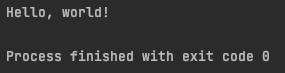
\includegraphics[width=0.5\textwidth]{jdk_ide_1}
  \caption{输出结果}
  \label{jdk_ide_1}
\end{figure}

接着,找到安装的JDK,如图\ref{jdk}所示,将其中的Unix可执行文件\verb|java|重命名为\verb|java1|。
\begin{figure}
  \centering
  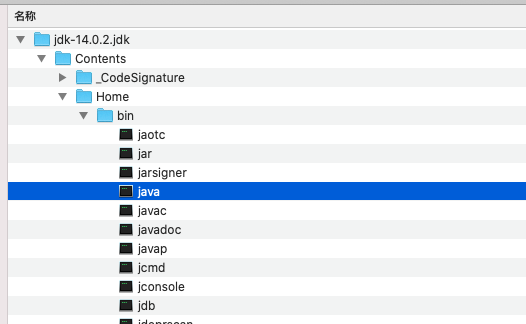
\includegraphics[width=0.5\textwidth]{jdk}
  \caption{安装的JDK}
  \label{jdk}
\end{figure}

然后,再次在IntelliJ IDEA中编译并运行,得到如图\ref{error_running}所示的报错,显示\verb|No such file or dictionary|,找不到JDK中的\verb|java|文件。
\begin{figure}
  \centering
  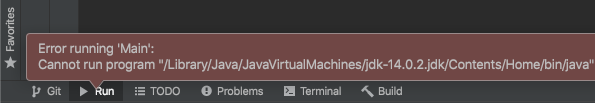
\includegraphics[width=0.5\textwidth]{error_running}
  \caption{报错}
  \label{error_running}
\end{figure}

最后,将文件\verb|java1|重新命名为\verb|java|,再次编译并运行,运行成功并输出。

实验过程中事件日志的截图如图\ref{event_log}所示。
\begin{figure}
  \centering
  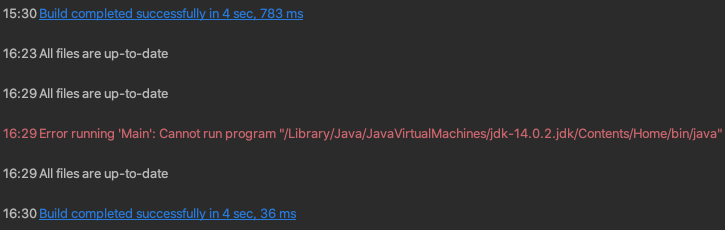
\includegraphics[width=0.5\textwidth]{event_log}
  \caption{实验事件日志}
  \label{event_log}
\end{figure}

\subsubsection*{实验结论}
\begin{enumerate}
  \item IDE是方便开发人员开发的集成开发工具,JDK是Java开发工具包。
  \item IDE能够帮助我们调用已安装的JDK提供的工具。若没有JDK或JDK损坏,则IDE不能顺利编译、解释。
\end{enumerate}

\subsection*{数据类型实验}

\subsubsection*{C++部分}

\paragraph{实验代码}
\lstset{language=c++}
\begin{lstlisting}
  #include <iostream>
  const int MAX = 20;
  int main(int argc, const char * argv[]) {
      short factorial = 1;
  //    unsigned short factorial = 1;
  //    int factorial = 1;
  //    unsigned int factorial = 1;
  //    long factorial = 1;
  //    unsigned long factorial = 1;
  //    long long factorial = 1;
  //    unsigned long long factorial = 1;
  //    float factorial = 1;
  //    double factorial = 1;
  //    long double factorial = 1;
      for (int n = 2; n < MAX; ++n)
      {
          factorial = factorial * n;
          std::cout << n << "! = " << factorial << std::endl;
      }
  }
\end{lstlisting}

\paragraph{输出结果}
改变变量\verb|factorial|的数据类型,观察输出。例如,对于\verb|short|类型的变量,得到如图\ref{cpp_short}所示的输出。因此,要使C++的\verb|short|类型变量不溢出,\verb|n|的最大值为7。
\begin{figure}
  \centering
  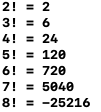
\includegraphics[width=0.3\textwidth]{cpp_short}
  \caption{C++/short类型}
  \label{cpp_short}
\end{figure}

经过实验,得到结果如表\ref{cpp_result}所示。
\begin{table}[]
  \centering
  \begin{tabular}{|c|c|}
  \hline
                     & $n_{\max}$ \\ \hline
  short              & 7          \\ \hline
  unsigned short     & 8          \\ \hline
  int                & 12         \\ \hline
  unsigned int       & 12         \\ \hline
  long               & 20         \\ \hline
  unsigned long      & 20         \\ \hline
  long long          & 20         \\ \hline
  unsigned long long & 20         \\ \hline
  float              & 34         \\ \hline
  double             & 170        \\ \hline
  long double        & 1754       \\ \hline
  \end{tabular}
  \caption{C++数据类型实验结果}
  \label{cpp_result}
\end{table}

\subsubsection*{Java部分}

\paragraph{实验代码}
\lstset{language=java}
\begin{lstlisting}
  public class Main {

    public static void main(String[] args) {
        final int MAX = 20;
        byte factorial = 1;
  //      short factorial = 1;
  //      int factorial = 1;
  //      long factorial = 1L;
  //      float factorial = 1f;
  //      double factorial = 1d;
        for (int n = 2; n < MAX; ++n)
        {
            factorial = (byte) (factorial * n);
            System.out.print(n);
            System.out.print("! = ");
            System.out.println(factorial);
        }
    }
}
\end{lstlisting}

改变变量\verb|factorial|的数据类型,观察输出。例如,对于\verb|byte|类型的变量,得到如图\ref{java_byte}所示的输出。因此,要使Java的\verb|byte|类型变量不溢出,\verb|n|的最大值为5。
\begin{figure}
  \centering
  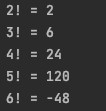
\includegraphics[width=0.3\textwidth]{java_byte}
  \caption{Java/byte类型}
  \label{java_byte}
\end{figure}

经过实验,得到结果如表\ref{java_result}所示。
\begin{table}[]
  \centering
  \begin{tabular}{|c|c|}
  \hline
         & $n_{\max}$ \\ \hline
  byte   & 5          \\ \hline
  short  & 7          \\ \hline
  int    & 12         \\ \hline
  long   & 20         \\ \hline
  float  & 34         \\ \hline
  double & 170        \\ \hline
  \end{tabular}
  \caption{Java数据类型实验结果}
  \label{java_result}
\end{table}

\subsection*{文件输出}
在上述代码后添加文件输出即可。

\subsubsection*{实验代码}
\lstset{language=java}
\begin{lstlisting}
  package com.company;

  import java.io.*;
  public class Main {
      public static void main(String[] args) {
          final int MAX = 100;
          double factorial = 1d;
          try {
              BufferedWriter out = new BufferedWriter(new FileWriter("factorial.csv"));
              for (int n = 1; n < MAX; ++n)
              {
                  factorial = factorial * n;
                  out.write(String.valueOf(n) + ',' + String.valueOf(factorial) + '\n');
              }
              out.close();
              System.out.println("Succeed to create the file.");
          } catch (IOException e)
          {
              System.out.println("Fail to create the file.");
          }
      }
  }
\end{lstlisting}

\subsubsection*{输出结果}
程序新建的csv文件可用Excel打开,如图\ref{factorial_csv}所示。
\begin{figure}
  \centering
  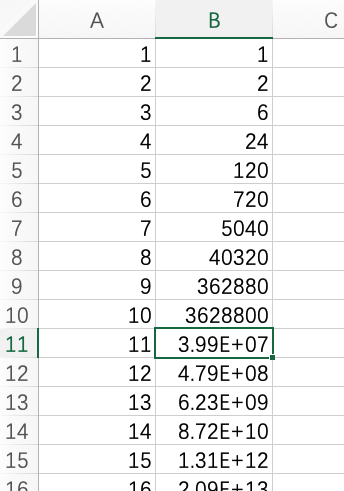
\includegraphics[width=0.3\textwidth]{factorial_csv}
  \caption{csv文件}
  \label{factorial_csv}
\end{figure}

\end{document}
